\chapter*{Preface}
This project has been constructed as part of the fourth semester project the by project group SW510E16 from Aalborg University, Software Engineering, from the period 2nd September to 21st December 2016 . \newline
The project is based on the \textit{Aalborg-model} study method, where problem and project based learning is the focus. The theme of this semester is to make an embedded system with real-time constraints. The project group chose to make a trash bin that should be able to catch the trash thrown at it. \newline

Thank the people who should be thanked for helping making the project, here. 
\newline
\newline
\newline
\newline

{\Huge\textbf{Signatures}}
\newline
\newline

\begin{table}[H]
	\centering
		\begin{tabular}{c c c}
			\underline{\phantom{mmmmmmmmmmmmmm}} & \underline{\phantom{mmmmmmmmmmmmmm}} & \underline{\phantom{mmmmmmmmmmmmmm}} \\
			Christian Dannesboe			& Frederik Børsting Lund 		& Karrar Al-Sami 			\\
			&&\\
			&&\\
			\underline{\phantom{mmmmmmmmmmmmmm}} & \underline{\phantom{mmmmmmmmmmmmmm}} & \underline{\phantom{mmmmmmmmmmmmmm}} \\
			Mark Kloch Haurum			& Lasse Lyngø Nielsen 		& Søren Lyng 				\\
			&&\\
			&&\\
		 																		
		\end{tabular}
\end{table}

\chapter*{Reading guide}
The sources in the report are being referred to by the Harvard citation method. This includes a last name and a publication year in the report, and in the \textit{\textbf{Bibliography}} chapter all the used sources are listed in alphabetical order. \newline
\textit{An example of a source in the text could be: \textbf{\citep{Servo}}.}
\newline
If the source is on the left side of a dot, then that source refers only to that sentence and if the source is on the right side of a dot, then it refers to the whole section. 

Figures and tables are referred to as a number. The number is determined by the chapter and the number of figure it appears as. \newline
\textit{For example: The first figure in a chapter will have the number \textbf{x.1}, where x is the number of the chapter. The next figure, will have the number \textbf{x.2}, etc.}
\newline
The listings of source code are also referred to as the tables and figures. 

Source code in the report are listed as code snippets, and they're not necessarily the same as the source code, meaning that code snippets may be shorter than the actual source code or missing comments from the source code. In order to show that, the use of the following three dots are used: \textit\textbf{{"..."}}, which means that some of the source code isn't listed in the code snippet, as it may be long and irrelevant. 

Throughout the report requirements are split into four colours with four different meanings. The colour blue refers to new requirements or focus requirements for that specific increment. The colour green refers to a requirement being fulfilled. Orange means that the requirement is fulfilled but has been changed. Red means that the requirement has been changed, but not yet fulfilled. 


\chapter*{Process model}
The process model is a meld of elements from both plan driven and agile development. The process is plan driven in so far as to include a clear goal of what the initial requirements of the system are. The process model is very agile in that, although there is a clear outline as to what the requirements are, these are incrementally approached, with a simple starting point becoming increasingly covering of the project vision through the subsequent increments.

The increments will be split up into four sections. Initially some of the already known requirements will be considered from previous increments and for the first increment from the analysis and hardware section, and these requirements will be the topic of the increment.
After the initial requirement consideration, an design phase follows which details the design and problem considerations preceding the implementation. The design phase is then followed by an implementation phase which will explain the implementation process. The final phase is an evaluation of the increment and will concern whether the requirements were fulfilled, or an requirement needs to be altered, or if an requirement will be continued in the following increment. The evaluated requirements from a increment will then become the starting point of the next increment. 

The process includes emphasis on a small group of individuals with tasks usually undertaken by two group members or more, which is to promote cooperation and attempt to avoid having a single individual involved in a task beyond their capabilities and to get a second opinion. This is also to ensure that information is quickly communicated and exchanged by group members. The process uses pair programming because it promotes better programming and is usually very motivating in socially engaging issues with cooperation of project members.

\begin{figure}[h]
\centering
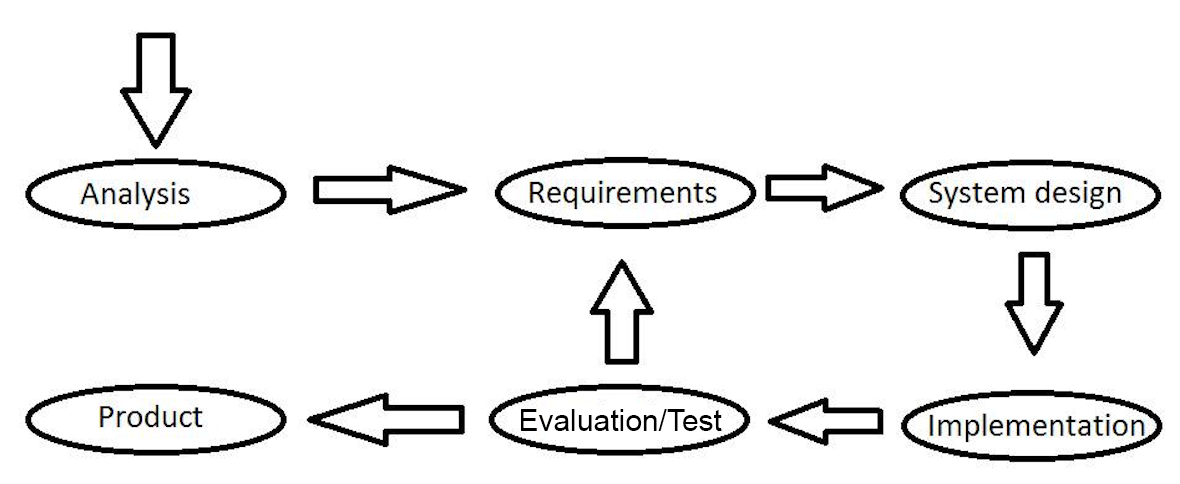
\includegraphics[scale=0.35]{billeder/process-model}
\caption{Process model used for the project}
\label{pm}
\end{figure}

